\section{NAM model (model ID: 41)}
The NAM model (fig.~\ref{fig:41_schematic}) is originally developed for use in Denmark \citep{Nielsen1973}. Here a small modification is made by replacing runoff routing equations of the form $\frac{1}{k}e^{-t/k}$ with the linear reservoirs these equations represent. The model has 6 stores and 10 parameters ($C_s$, $C_{if}$, $L^*$, $C_{L1}$, $U^*$, $C_{of}$, $C_{L2}$, $K_0$, $K_1$ and $K_b$). The model aims to represent:

\begin{itemizecompact}
\item Snow accumulation and melt;
\item Interflow when total soil moisture exceeds a threshold;
\item Separation of saturation excess flow into overland flow and infiltration;
\item Baseflow from groundwater.;
\end{itemizecompact}

\subsection{MARRMoT model name}
m\_41\_nam\_10p\_6s \\

% Equations
\subsection{Model equations}

% Model layout figure
{ 																	% This ensures it doesn't warp text further down
\begin{wrapfigure}{l}{6cm}
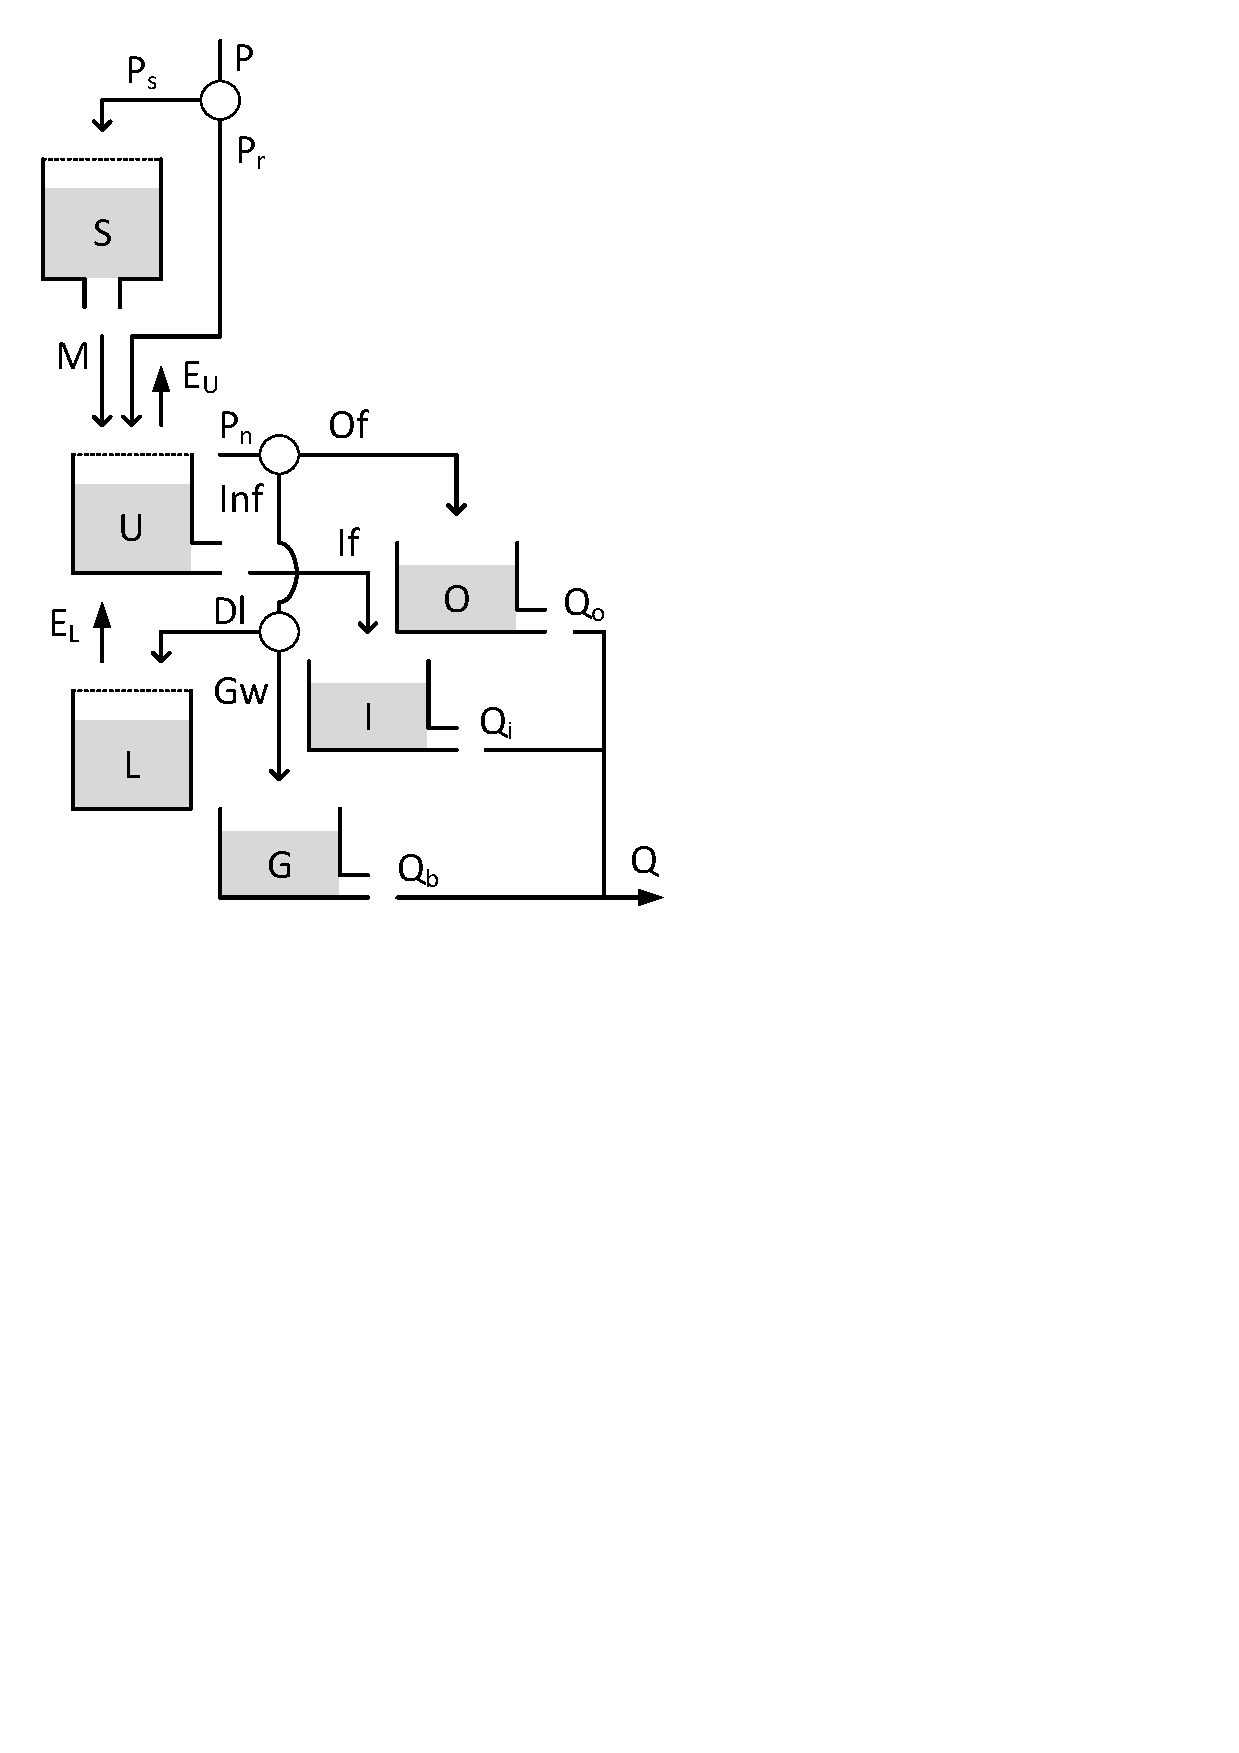
\includegraphics[trim=1cm 14cm 7cm 1cm,width=7cm,keepaspectratio]{./AppA_files/41_schematic.pdf}
\caption{Structure of the NAM model} \label{fig:41_schematic}
\end{wrapfigure}

\begin{align}
	\frac{dS}{dt} &= P_s-M \\
	P_s &= \begin{cases}
		P, &\text{if } T \leq 0 \\
		0, & \text{otherwise} \\
	\end{cases} \\
	M &= 
	\begin{cases}
		C_s*T, & \text{if } T > 0 \\
		0, & \text{otherwise}
	\end{cases}
\end{align}

Where $S$ is the current snow storage [mm], $P_s$ $[mm/d]$ the precipitation that falls as snow and M the snowmelt $[mm/d]$ based on a degree-day factor ($c_s$, [mm/\degree C/d]). The freezing point of $0^o$ [C] is used as a threshold for snowfall and melt.

} % end of wrapfigure fix

\begin{align}
	\frac{dU}{dt} &= P_r + M -E_U - If - P_n\\
	P_r &= \begin{cases}
		P, &\text{if } T > 0 \\
		0, & \text{otherwise} \\
	\end{cases} \\
	E_U &= \begin{cases}
		E_p, &\text{if } U > 0 \\
		0, &\text{otherwise} \\
	\end{cases} \\
	If &= \begin{cases}
		C_{if}*\frac{L/L^*-C_{L1}}{1-C_{L1}}U, &\text{if } L/L^* > C_{L1}\\
		0, &\text{otherwise}\\
	\end{cases}\\
	P_n &= \begin{cases}
		(P_r + M), &\text{if } U = U^*\\
		0, &\text{otherwise}\\
	\end{cases}	
\end{align}

Where U [mm] is the current storage in the upper zone, refilled by precipitation as rain $P_r$ $[mm/d]$ and snowmelt $M$, and drained by evaporation $E_U$ $[mm/d]$, interflow $If$ $[mm/d]$ and net precipitation $P_n$ $[mm/d]$. 
$P_r$ occurs only when the current temperature exceeds the threshold of $0^o$C. 
$E_U$ occurs at the potential rate $E_p$ whenever possible. 
$If$ occurs only if the fractional storage in the lower zone $L/L^*$ ($L$ is current lower zone storage, $L^*$ is lower zone maximum storage) exceeds a threshold $C_{L1}$ [-]. 
$If$ is scaled by the current deficit in the lower zone and a uses runoff coefficient $C_{if}$ [-]. 
$P_n$ occurs only when the upper zone exceeds its maximum storage capacity $U^*$ [mm].

\begin{align}
	\frac{dL}{dt} &= Dl - E_t \\
	Dl &= (P_n - Of)\left(1-\frac{L}{L^*}\right)\\
	Of &= \begin{cases}
		C_{of}*\frac{L/L^*-C_{L2}}{1-C_{L2}}*P_n, &\text{if } L/L^* > C_{L2}\\
		0, &\text{otherwise}\\
	\end{cases}\\
	E_t &=\begin{cases}
		 \frac{L}{L^*}E_p, &\text{if } U = 0\\
		0, &\text{otherwise}\\
	\end{cases}
\end{align}
  
Where $L$ [mm] is the current storage in the lower zone, refilled by a fraction of infiltration $Dl$ $[mm/d]$ and drained by evaporation $E_t$ $[mm/d]$. $Dl$ is calculated as a fraction of infiltration $P_n -Of$, dependent on the current deficit in the lower zone. 
Note that with the current formulation $Dl$ might be larger than the lower zone deficit $L^*-L$ and a constraint of the form $Dl \leq L^*-L$ is needed.
 Overland flow $Of$ $[mm/d]$ is a fraction of $P_n$ determined using the relative storage in the lower zone $L/L^*$ and two coefficients $C_{of}$ [-] and $C_{L2}$ [-]. 
$E_t$ occurs only when the upper zone is empty, and at a reduced rate that uses the relative storage in the lower zone.

\begin{align}
	\frac{dO}{dt} &= Of - Q_o\\
	Q_o &= K_0 * O 
\end{align}

Where $O$ [mm] is the current storage in the overland flow routing store.
$Q_o$ is the routed overland flow, using time coefficient $K_0$ $[d^{-1}]$.

\begin{align}
	\frac{dI}{dt} &= If - Q_i\\
	Q_i &= K_1 * I 
\end{align}

Where $I$ [mm] is the current storage in the interflow routing store.
$Q_i$ is the routed interflow, using time coefficient $K_1$ $[d^{-1}]$.

\begin{align}
	\frac{dG}{dt} &= Gw - Q_b\\
	Gw &= (P_n-Of)\left(\frac{L}{L^*}\right)\\
	Q_b &= K_b * O 
\end{align}

Where $G$ [mm] is the current storage in the overland flow routing store, refilled by groundwater flow $Gw$ $[mm/d]$.
$Q_b$ is the routed baseflow, using time coefficient $K_b$ $[d^{-1}]$. Total flow:

\begin{align}
	Q &= Q_o+Q_i+Q_b
\end{align}


\subsection{Parameter overview}
% Table generated by Excel2LaTeX from sheet 'Sheet1'
\begin{table}[htbp]
  \centering
    \begin{tabular}{lll}
    \toprule
    Parameter & Unit  & Description \\
    \midrule
    $C_s$ & $mm~^oC^{-1}~d^{-1}$ & Degree-day factor \\
    $C_{if}$ & $d^{-1}$ & Runoff coefficient \\
    $L^*$ & $mm$  & Maximum lower zone storage \\
    $C_{L1}$ & $-$   & Fractional threshold for interflow generation \\
    $U^*$ & $mm$  & Maximum upper zone storage \\
    $C_{of}$ & $d^{-1}$ & Runoff coefficient \\
    $C_{L2}$ & $-$   & Fractional threshold for overland flow generation \\
    $K_0$ & $d^{-1}$ & Runoff coefficient \\
    $K_1$ & $d^{-1}$ & Runoff coefficient \\
    $K_b$ & $d^{-1}$ & Runoff coefficient \\
    \bottomrule
    \end{tabular}%
  \label{tab:addlabel}%
\end{table}%

